\begin{tikzpicture}
\node at (0,0) {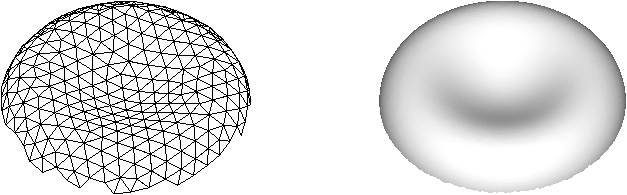
\includegraphics[width=25em]{network2continuum.pdf}};
\node[text width=10em] at (-3,2.2) {\bf 弹簧常数, 弯曲常数, 体积约束, 面积约束};
\node[text width=10em] at ( 3,2.2) {\bf 剪切模量, 压缩模量, 杨氏模量, 弯曲刚度};
\node[text width=5em] at (-2.8,-2) {\bf 粒子模型};
\node[text width=5em] at ( 2.8,-2) {\bf 连续模型};
\draw[very thick, <->, >=stealth'] (-1,2.2) -- (1, 2.2);
\draw[very thick, <->, >=stealth'] (-0.8,0) -- (0.8, 0);
\draw[very thick, <->, >=stealth'] (-1.2,-2) -- (1.2, -2);
\end{tikzpicture}
